\documentclass[]{article}

\usepackage[utf8]{inputenc}
\usepackage{amsmath}
\usepackage{amssymb}
\usepackage{amsthm}
\usepackage{amsfonts}
\usepackage{graphicx}
\usepackage{capt-of}
\usepackage{listings}
\usepackage{siunitx}
\usepackage[section]{placeins}
\usepackage{multicol}
\usepackage[a4paper, portrait, margin=1in]{geometry}
\usepackage{float}
\usepackage{caption}
\usepackage{subcaption}
\usepackage{xcolor}

% Solarized colour scheme for listings
\definecolor{solarized@base03}{HTML}{002B36}
\definecolor{solarized@base02}{HTML}{073642}
\definecolor{solarized@base01}{HTML}{586e75}
\definecolor{solarized@base00}{HTML}{657b83}
\definecolor{solarized@base0}{HTML}{839496}
\definecolor{solarized@base1}{HTML}{93a1a1}
\definecolor{solarized@base2}{HTML}{EEE8D5}
\definecolor{solarized@base3}{HTML}{FDF6E3}
\definecolor{solarized@yellow}{HTML}{B58900}
\definecolor{solarized@orange}{HTML}{CB4B16}
\definecolor{solarized@red}{HTML}{DC322F}
\definecolor{solarized@magenta}{HTML}{D33682}
\definecolor{solarized@violet}{HTML}{6C71C4}
\definecolor{solarized@blue}{HTML}{268BD2}
\definecolor{solarized@cyan}{HTML}{2AA198}
\definecolor{solarized@green}{HTML}{859900}

\lstset{language=C++,
        basicstyle=\footnotesize\ttfamily,
        numbers=left,
        numberstyle=\footnotesize,
        tabsize=2,
        breaklines=true,
        escapeinside={@}{@},
        numberstyle=\tiny\color{solarized@base01},
        keywordstyle=\color{solarized@green},
        stringstyle=\color{solarized@cyan}\ttfamily,
        identifierstyle=\color{solarized@blue},
        commentstyle=\color{solarized@base01},
        emphstyle=\color{solarized@red},
        frame=single,
        rulecolor=\color{solarized@base2},
        rulesepcolor=\color{solarized@base2},
        showstringspaces=false
}



% Oppgavenummerering %
\renewcommand\thesection{Task \arabic{section}}
\renewcommand\thesubsection{\alph{subsection})}
\renewcommand\thesubsubsection{\alph{subsection}.\alph{subsubsection})}

% Bevis
\newcommand\TombStone{\rule{.5em}{.5em}}
\renewcommand\qedsymbol{\TombStone}

\title{\Huge{Assignment 3} \\ \Large{TDT4195 – Visual Computing Fundamentals}}
\author{Sigurd Totland | MTTK}

\begin{document}
\maketitle
\begin{multicols}{2}
\section{The Eagle has Landed}
\subsection{}
We begin by simply creating a \texttt{Mesh} object from \texttt{lunarsurface.obj} and sending the vertex, colour, and index vectors into the \texttt{createVAO} function. As expected, the lunar surface renders correctly, albeit without any colors at this time, so it is completely white as shown in figure \ref{fig:white-surface} below.
\begin{figure}[H]
\centering
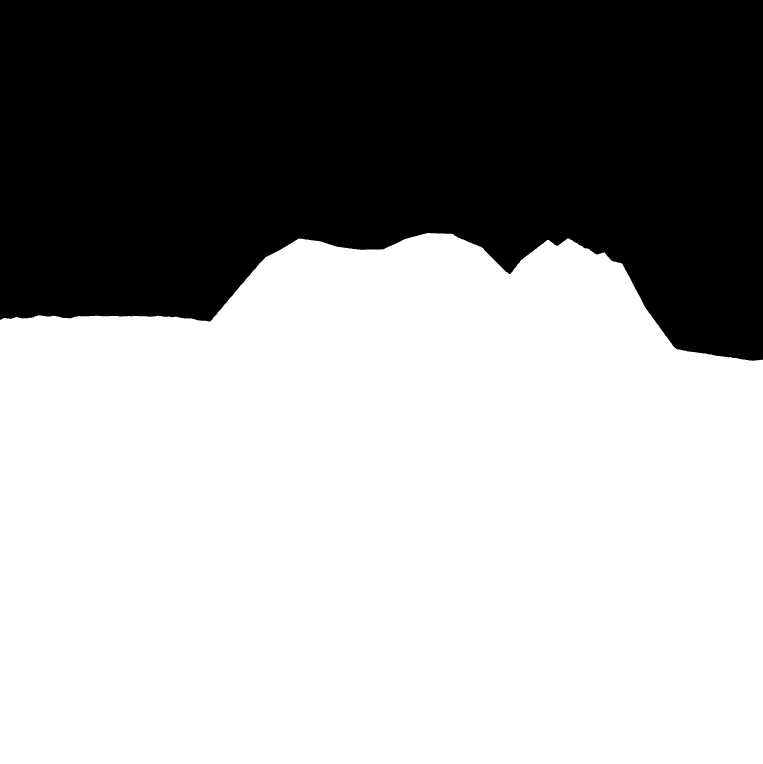
\includegraphics[width=0.5\columnwidth]{white-surface}
\caption{Lunar surface without any coloring}
\label{fig:white-surface}
\end{figure}

\setcounter{subsection}{2}
\subsection{}
In this task and the previous, we add a third VBO to hold the normals and pass these values through the vertex shader into the fragment shader. Setting the fragment color equal to the x, y, and z components of each normal vector yields a predominantly green surface as shown in figure \ref{fig:green-surface} below.
\begin{figure}[H]
\centering
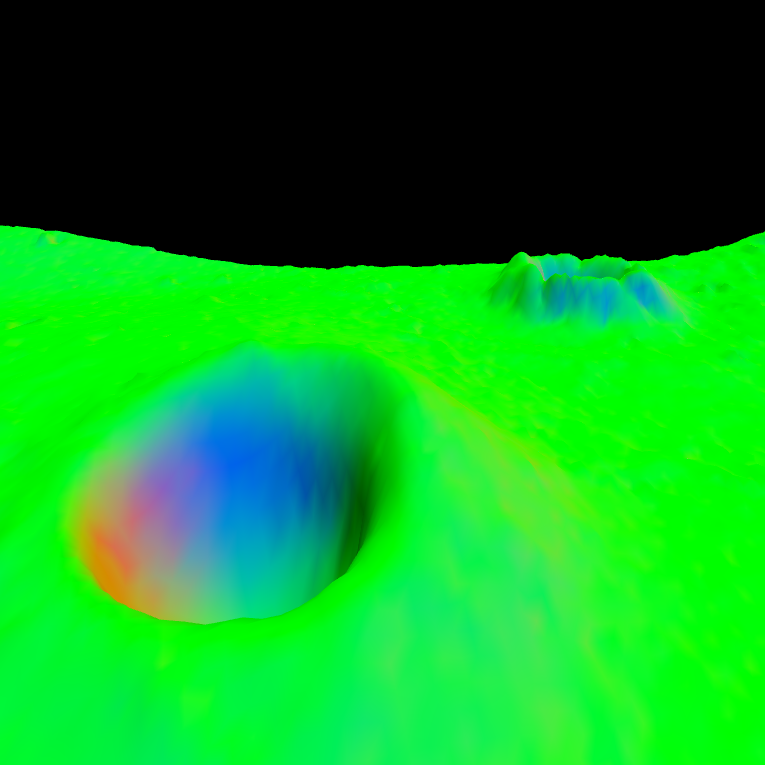
\includegraphics[width=0.5\columnwidth]{green-surface}
\caption{Lunar surface colored by directly inserting the surface normal values}
\label{fig:green-surface}
\end{figure}
We notice how green color corresponds to upward pointing normals, whereas red and blue are for more sideways surfaces.

\subsection{}
Inserting the Lambertian illumination model,
\begin{equation}\begin{aligned}
\text{color} * \max(0, \hat{\mathbf{n}} \cdot (- \hat{\mathbf{l}})),
\end{aligned}\end{equation}
where $\hat{\mathbf{n}}$ is the surface normal and $\hat{\mathbf{l}}$ is the normalized lighting direction the surface becomes a \textit{Lambertian surface}. Coloring the surface a pure white results in the following (quite convincing) scene, clearly showing that the surface is indeed lit. (Figure \ref{fig:lambert-surface}).
\begin{figure}[H]
\centering
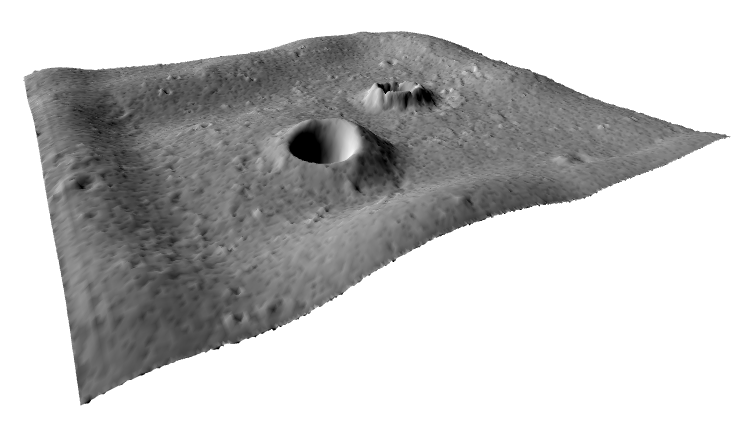
\includegraphics[width=0.5\columnwidth]{lambert-surface}
\caption{Lunar surface with Lambertian shading}
\label{fig:lambert-surface}
\end{figure}
\end{multicols}
\appendix
\section{C++ snippets}
\begin{lstlisting}[language={C++}, caption={Vertices for 6 triangles}, label={lst:6_tris_1}]
// hello world
\end{lstlisting}

\end{document}

